% This is text associated with the open textbook "Open Electromagnetics"
% See immediately below for author, date
% This work is licensed under the Creative Commons Attribution-ShareAlike 4.0 International License. (CC BY SA 4.0) 
% To view a copy of the license, visit http://creativecommons.org/licenses/by-sa/4.0/

%ORB TITLE Inductance
%ORB AUTHOR 0        # S.W. Ellingson, Virginia Tech (ellingson@vt.edu)
%ORB DATE 20180806   # yyyymmdd
%ORB ABSTRACT Inductance

\label{m0123_Inductance} % <-- Must match name of this file and module directory name.  Don't mess with this!
\index{inductance|(}

Current creates a magnetic field, which subsequently exerts force on other current-bearing structures.
For example, the current in each winding of a coil exerts a force on every other winding of the coil.
If the windings are fixed in place, then this force is unable to do work (i.e., move the windings), so instead the coil stores potential energy.
This potential energy can be released by turning off the external source.
When this happens, charge continues to flow, but is now propelled by the magnetic force.  
The potential energy that was stored in the coil is converted to kinetic energy and subsequently used to redistribute the charge until no current flows.
At this point, the inductor has expended its stored energy.
To restore energy, the external source must be turned back on, restoring the flow of charge and thereby restoring the magnetic field.
 
Now recall that the magnetic field is essentially defined in terms of the force associated with this potential energy; i.e., ${\bf F} = q{\bf v} \times {\bf B}$ where $q$ is the charge of a particle comprising the current, ${\bf v}$ is the velocity of the particle, and ${\bf B}$ is magnetic flux density (Section~\ref{m0003_Magnetic_Flux_Density}).
So, rather than thinking of the potential energy of the system as being associated with the magnetic force applied to current, it is equally valid to think of the potential energy as being stored in the magnetic field associated with the current distribution.
The energy stored in the magnetic field depends on the geometry of the current-bearing structure and the permeability of the intervening material because the magnetic field depends on these parameters. 

The relationship between current applied to a structure and the energy stored in the associated magnetic field is what we mean by \emph{inductance}.
We may fairly summarize this insight as follows:
%
%ORB HIGHLIGHT
\begin{mdframed}[backgroundcolor=yellow!20,nobreak=true] 
Inductance 
\index{inductance!definition}
is the ability of a structure to store energy in a magnetic field.
\end{mdframed}
%
%ORB HIGHLIGHT
\begin{mdframed}[backgroundcolor=yellow!20,nobreak=true] 
The inductance of a structure depends on the geometry of its current-bearing structures and the permeability of the intervening medium.
\end{mdframed}

Note that inductance does \emph{not} depend on current, which we view as either a stimulus or response from this point of view.
The corresponding response or stimulus, respectively, is the magnetic flux 
\index{magnetic flux|see{flux, magnetic}}
\index{flux!magnetic}
associated with this current.
This leads to the following definition:
%
\begin{equation}
L = \frac{\Phi}{I} ~~\mbox{(single linkage)}
\label{m0123_Ldef}
\end{equation} 
%
\index{linkage}
\index{flux linkage!see{linkage}}
where $\Phi$ (units of Wb) is magnetic flux, $I$ (units of A) is the current responsible for this flux, and $L$ (units of H) is the associated inductance.
(The ``single linkage'' caveat will be explained below.)
In other words, a device with high inductance generates a large magnetic flux in response to a given current, and therefore stores more energy for a given current than a device with lower inductance.

To use Equation~\ref{m0123_Ldef} we must carefully define what we mean by ``magnetic flux'' in this case.
Generally, magnetic flux is magnetic flux density (again, ${\bf B}$, units of Wb/m$^2$) integrated over a specified surface ${\mathcal S}$, so
%
\begin{equation}
\Phi = \int_{\mathcal S}{\bf B}\cdot d{\bf s}
\end{equation}
%
where $d{\bf s}$ is the differential surface area vector, with direction normal to ${\mathcal S}$.
However, this leaves unanswered the following questions: Which ${\mathcal S}$, and which of the two possible normal directions of $d{\bf s}$?
For a meaningful answer, ${\mathcal S}$ must uniquely associate the magnetic flux to the associated current. 
Such an association exists if we require the current to form a closed loop.
This is shown in Figure~\ref{m0123_fFluxCurrent}.
Here ${\mathcal C}$ is the closed loop along which the current flows, ${\mathcal S}$ is a surface bounded by ${\mathcal C}$, and the direction of $d{\bf s}$ is defined according to the right-hand rule
\index{right-hand rule!Stokes' theorem}
of Stokes' Theorem 
\index{Stokes' theorem}
(Section~\ref{m0051_Stokes_Theorem}).
Note that ${\mathcal C}$ can be a closed loop of \emph{any} shape; i.e., not just circular, and not restricted to lying in a plane.
Further note that ${\mathcal S}$ used in the calculation of $\Phi$ can be \emph{any} surface bounded by ${\mathcal C}$.
This is because magnetic field lines form closed loops such that any one magnetic field line intersects any open surface bounded by ${\mathcal C}$ exactly once. 
Such an intersection is sometimes called a ``linkage.''
So there we have it -- we require the current $I$ to form a closed loop, we measure the magnetic flux through this loop using the sign convention of the right-hand rule, and the ratio is the inductance.
%
\begin{figure}
\begin{center}
\pdftooltip{{  % note double braces
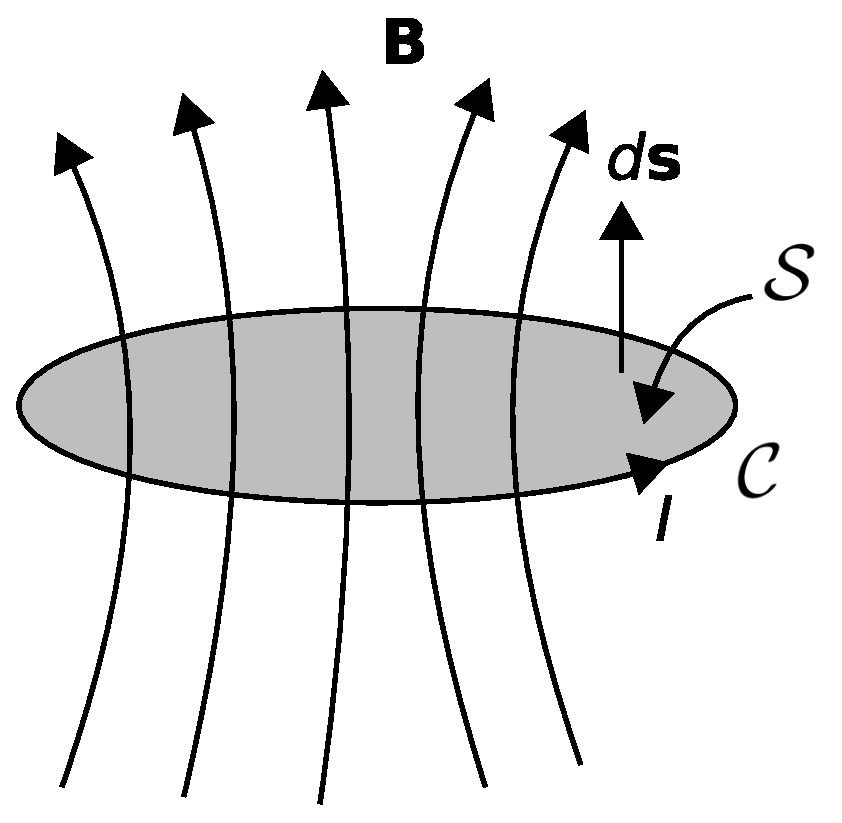
\includegraphics[width=2in]{modules/m0123_fFluxCurrent.eps}
% https://commons.wikimedia.org/wiki/File:M0123_fFluxCurrent.svg
}}{A circular surface, S, bounded by closed path C. On C, an arrow labeled I is pointing in a counterclockwise direction, following Stokes' Theorem. A vector labeled ds points out of the surface S. Five vectors labeled B go through the middle of S and point upward: The left three are curved to the left, and the right two are curved to the right.}
\end{center} 
\centerline{\scriptsize 
\copyright~\hyperref[m0123_fFluxCurrent_Credit]{K.\ Kikkeri} 
\href{https://creativecommons.org/licenses/by-sa/4.0/}{CC BY~SA 4.0} 
} 
\caption{
\label{m0123_fFluxCurrent}
Association between a closed loop of current and the associated magnetic flux.
}
\end{figure}

Many structures consist of multiple such loops -- the coil 
\index{coil}
is of course one of these.
In a coil, each winding carries the same current, and the magnetic fields of the windings add to create a magnetic field, which grows in proportion to the winding density (Section~\ref{m0120_Magnetic_Field_of_a_Coil}).
The magnetic flux density inside a coil is proportional to the number of windings, $N$, so 
the flux $\Phi$ in Equation~\ref{m0123_Ldef} should properly be indicated as $N\Phi$.
Another way to look at this is that we are counting the number of times the same current is able to generate a unique set of magnetic field lines that intersect ${\mathcal S}$.
%For this reason it is common to refer to the quantity $N\Phi$ as ``flux linkages''.

Summarizing, our complete definition for inductance is
%
\begin{equation}
\boxed{
L = \frac{N\Phi}{I}~~\mbox{(identical linkages)}
}
\label{m0123_Ldef2}
\end{equation} 
%
%ORB HIGHLIGHT
\begin{mdframed}[backgroundcolor=yellow!20,nobreak=true] 
An engineering definition of inductance 
\index{inductance!definition}
is Equation~\ref{m0123_Ldef2}, with the magnetic flux defined to be that associated with a single closed loop of current with sign convention as indicated in Figure~\ref{m0123_fFluxCurrent}, and $N$ defined to be the number of times the same current $I$ is able to create that flux.
\end{mdframed}
%
What happens if the loops have different shapes?  For example, what if the coil is not a cylinder, but rather cone-shaped? (Yes, there is such a thing -- see ``Additional Reading'' at the end of this section.)  In this case, one needs a better way to determine the factor $N\Phi$ since the flux associated with each loop of current will be different.  
However, this is beyond the scope of this section.  

An \emph{inductor} 
\index{inductor}
is a device that is designed to exhibit a specified inductance.
We can now make the connection to the concept of the inductor as it appears in elementary circuit theory.
First, we rewrite Equation~\ref{m0123_Ldef2} as follows:
%
\begin{equation}
I = \frac{N\Phi}{L}
\end{equation} 
%
Taking the derivative of both sides of this equation with respect to time, we obtain:
%
\begin{equation}
\frac{d}{dt}I = \frac{N}{L}\frac{d}{dt}\Phi
\label{m0123_edIdt}
\end{equation} 
%
Now we need to reach beyond the realm of magnetostatics for just a moment. 
Section~\ref{m0055_Faradays_Law} (``Faraday's Law'') shows that the change in $\Phi$ associated with a change in current %non-zero $dI/dt$ 
results in the creation of an electrical potential equal to $-Nd\Phi/dt$ realized over the loop ${\mathcal C}$.  
In other words, the terminal voltage $V$ is $+Nd\Phi/dt$, with the change of sign intended to keep the result consistent with the sign convention relating current and voltage in passive devices.
Therefore, $d\Phi/dt$ in Equation~\ref{m0123_edIdt} is equal to $V/N$.
Making the substitution we find:
%
\begin{equation}
V = L\frac{d}{dt}I
\label{m0125_eLCT} 
\end{equation}
%
This is the expected relationship from elementary circuit theory.

Another circuit theory concept related to inductance is \emph{mutual inductance}.  
\index{mutual inductance}
Whereas inductance relates changes in current to instantaneous voltage in the same device (Equation~\ref{m0125_eLCT}), mutual inductance relates changes in current in one device to instantaneous voltage in a \emph{different} device.  This can occur when the two devices are coupled (``linked'') by the same magnetic field.  For example, \emph{transformers}
\index{transformer}
(Section~\ref{m0031_Transformers_Principle_of_Operation}) typically consist of separate coils that are linked by the same magnetic field lines.  The voltage across one coil may be computed as the time-derivative of current on the other coil times the mutual inductance.   

Let us conclude this section by taking a moment to dispel a common misconception about inductance.  
The misconception pertains to the following question.  If the current does not form a closed loop, what is the inductance?
For example, engineers sometimes refer to the inductance of a pin or lead of an electronic component.
A pin or lead is not a closed loop, so the formal definition of inductance given above -- ratio of magnetic flux to current -- does not apply.
The broader definition of inductance -- the ability to store energy in a magnetic field -- does apply, but this is \emph{not} what is meant by ``pin inductance'' or ``lead inductance.''  
What is actually meant is the imaginary part of the impedance of the pin or lead -- i.e., the reactance -- expressed as an equivalent inductance.
In other words, the reactance of an inductive device is positive, so any device that also exhibits a positive reactance can be viewed from a circuit theory perspective as an equivalent inductance.  
This is not referring to the storage of energy in a magnetic field; it merely means that the device can be modeled as an inductor in a circuit diagram.
In the case of ``pin inductance,'' the culprit is not actually inductance, but rather skin effect 
\index{skin effect}
(see ``Additional References'' at the end of this section).
Summarizing: 
%
%ORB HIGHLIGHT
\begin{mdframed}[backgroundcolor=yellow!20,nobreak=true] 
Inductance implies positive reactance, but positive reactance 
\index{reactance}
does not imply the physical mechanism of inductance. 
\end{mdframed}

%------------------------------------
 
{\bf Additional Reading:}
\begin{itemize}
\item ``\href{https://en.wikipedia.org/wiki/Inductance}{Inductance}'' on Wikipedia.
\item ``\href{https://en.wikipedia.org/wiki/Inductor}{Inductor}'' on Wikipedia.
\item T.A.\ Winslow, ``\href{https://doi.org/10.1109/MMW.2005.1418000}{Conical Inductors for Broadband Applications},'' \emph{IEEE Microwave Mag.}, Vol.~6, No.~1, Mar 2005, pp.~68--72.
\item ``\href{https://en.wikipedia.org/wiki/Skin_effect}{Skin Effect}'' on Wikipedia.
\end{itemize}

\index{inductance|)}
